%*****************************************
\chapter{Preliminaries}\label{ch:Preliminaries}
%*****************************************
%\setcounter{figure}{10}
% \NoCaseChange{Homo Sapiens}

\section{The Root of All Good: Hoare Triples}
In 1969, C.A.R. Hoare published his famous article \textit{An Axiomatic Basis for Computer Programming}~\cite{Hoare69} to explore the logic of computer programs use axioms and inference rules to prove the properties of programs. 
This system is known referred as \define{Hoare Triples}. 
He introduced \imptt{sufficient} preconditions that will guarantee correct results but does not rule out non-termination. 
A selection of the axioms and rules are shown in \autoref{tab:hoare}. \footnote{We omit the symbol $\vdash$ in front of a Hoare Triple, which denotes ``valid/provable'', for better readability. }\footnote{Nondeterminism was not considered in the original paper, so we treat the programs here as deterministic. } 

\begin{table}[ht]\centering
    \begin{tabular}{ll}
      \hline 
      \textbf{Axiom of Assignment}     &  \hoare{F[x/e]}{x:=e}{F}   \\
      \textbf{Rules of Consequence}   &  If \hoare{G}{C}{F} and $F\Rightarrow P$ then \hoare{G}{C}{P} \\
                                      &  If \hoare{G}{C}{F} and $P\Rightarrow G$ then \hoare{P}{C}{F} \\
      \textbf{Rule of Composition}   &  If \hoare{G}{C_1}{F_1} and \hoare{F_1}{C_2}{F} then \hoare{G}{C_1;C_2}{F} \\
      \textbf{Rule of Iteration}  &  If $F\wedge$(\hoare{G}{C}{F}) then \hoare{F}{\text{while } B \text{ do } C }{\neg B \wedge F}  \\
      % \textbf{Rule of Condition}   &  $wp.C_1.(wp.C_2.F)$\\
      \hline
    \end{tabular}
    \caption{Valid Hoare Triples}
    \label{tab:hoare}
\end{table}

\mathl{\{F[x/e]\}} is obtained by substituting occurrences of $x$ by $e$. 

Semantically, a Hoare Triple \hoare{G}{C}{F} is said to be valid for (partial) correctness, if the execution of the program $C$ with an initial state satisfying the precondition $G$ leads to a final state that satisfies the postcondition $F$, provided that the program terminates. 
\autoref{fig:hoare} illustrates a valid Hoare Triple, $\Sigma$ represents the set of all states, the section denoted with $G$ includes the states that satisfy the predicate $G$. The arrow from left to write denotes the execution of the program $C$. 

\begin{figure}[ht]\centering
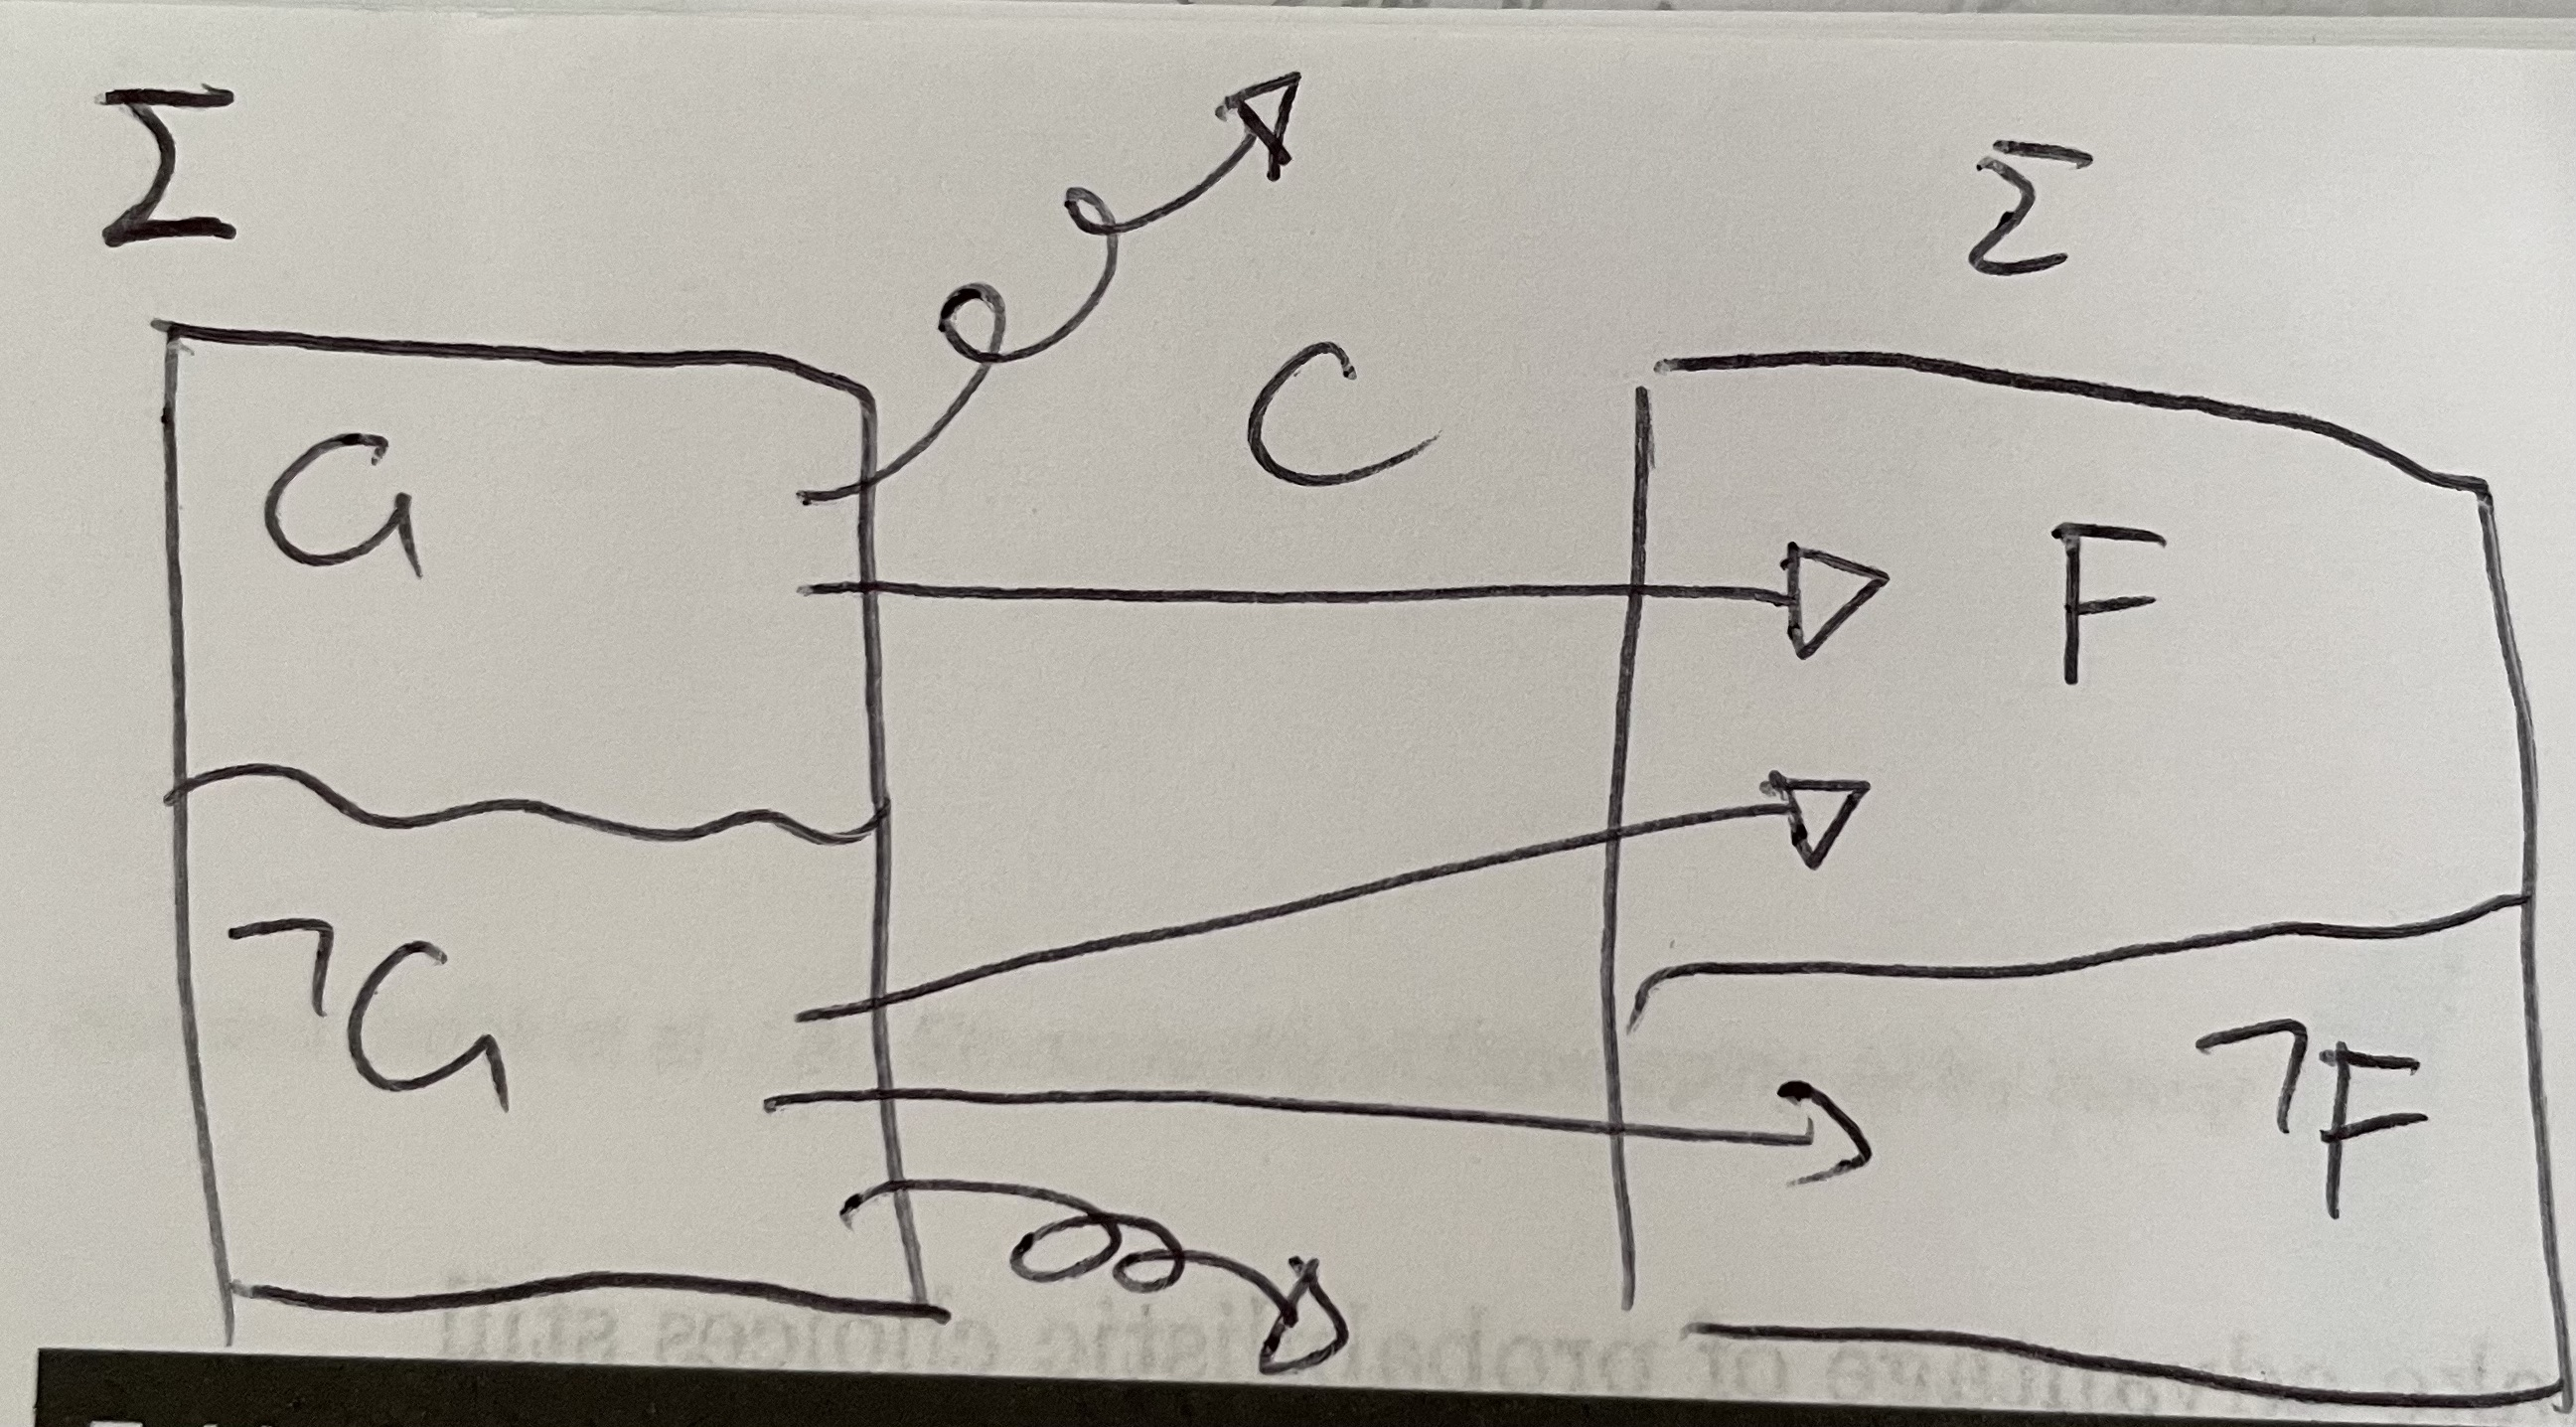
\includegraphics[width=0.5\textwidth]{image/hoare.jpg}
\caption{Valid Hoare Triple (Deterministic)}
\label{fig:hoare}
\end{figure}
\todo{Digitize image, also add program C. }

The proof system built by Hoare's rules is sound, expressive, yet incomplete.~\cite{Apt81}
A sensible advancement would be to find the \imptt{necessary and sufficient} preconditions that grant us the post-properties, i.e. to eliminate the arrows from $\neg G$ to $F$ in \autoref{fig:hoare}. 


\section{Guarded Command Language}
We use Dijkstra's (non-deterministic) \define{guarded command language (GCL)}~\cite{Dijkstra75} to conceptualize a computer program and to include non-determinism.
For better understanding, we use an equivalent
\footnote{Specifically, $if\ (\varphi)\ \{C_1\}\ else\ \{C_2\} $ is equivalent to
$if\ \varphi \to C_1$ $[]$ $\neg\varphi \to C_2\ fi$ in Dijkstra's original style\cite{Dijkstra75}; $\{C_1\}\square \{C_2\}$ is equivalent to $if\ true\to C_1$ $[]$ $true\to C_2\ fi$.} 
form of nGCL that is similar to modern pseudo-code:

\begin{table}[h!]\centering
    \begin{tabular}{cl}
    $C\ ::=$ &  $x:= e   \ \ \mid \ \  C;C  \ \ \mid \ \   \{C\}\square \{C\}  \ \ \mid \ \  if\ (\varphi)\ \{C\}\ else\ \{C\} 
     \ \ \mid\ \  while\ (\varphi)\ \{C\}$ \\ 
  &$\mid skip \mid diverge$
    \end{tabular}
\end{table}



\section{Weakest Precondition}
We define the \define{weakest precondition} transformer structurally in lambda-calculus style\footnote{For example, $wp.C.F$ can be seen as $wp(C,F)$ in ``typical'' style, where $wp$ is treated as a function that has two parameters. The advantage of lambda-calculus style is scalability, we can simply extend the aforementioned function like $wp.C.F.\sigma$ where $\sigma$ means the initial state. Here $wp$ is treated as a function that has three parameters, if we were to write it in the ``typical'' style. It is then questionable whether we changed the type of $wp$. } as follows: 

\begin{table}[h!]\centering
    \begin{tabular}{ll}
      \textbf{C}&\textbf{wp.C.F}    \\ \hline
      $skip$&   $F$   \\
      $diverge$&  $false$\\
      $x:= e $&  $F[x/e]$\\
      $C_1;C_2$&  $wp.C_1.(wp.C_2.F)$\\
      $if\ (\varphi)\ \{C_1\}\ else\ \{C_2\} $&  $(\varphi\wedge wp.C_1.F)\vee(\neg\varphi\wedge wp.C_2.F)$\\
      $\{C_1\}\square \{C_2\}$ & $wlp.C_1.F\vee wlp.C_2.F$ \\
      $while\ (\varphi)\ \{C'\}$&  $lfp\ X.(\neg\varphi\wedge F)\vee(\varphi\wedge wp.C'.X)$\\
    \end{tabular}
    \caption{The Weakest Precondition Transformer}
\end{table}

\mathl{F[x/e]} is $F$ where every occurrence of $x$ is syntactically replaced by $e$. 

\mathl{lfp\ X. f} is the least fixed point of function $f$ with variable $X$. 

Let \mathl{$\Phi(X):=(\neg\varphi\wedge F)\vee(\varphi\wedge wp.C'.X)$} be the characteristic function. 

To justify this definition, we must first clarify the intended semantics/meaning of the wp-transformer. 
Let \mathl{\exec C} denote the \define{execution} of program $C$, \mathl{\exec C.\sigma} denote the set of final states that \imptt{can} occur after the execution of $C$. 

(A state is a function that maps a program variable to a value. The set of \define{states} is denoted by \mathl{\Sigma=\{\sigma \mid \sigma: Vars\to Vals\}}. )

If $C$ is deterministic, then $\exec C.\sigma$ is a set of a single state, either a final state $\sigma'$ or $\bot$, if the execution does not terminate. 
If $C$ is non-deterministic, $\exec C.\sigma$ can be a set with multiple elements, since multiple final states can be possible. 

The weakest precondition $wp.C.F$ is then 
\todo{Justify all the definitions except while. }

\todo{Explain least point iteration from bottom. }

\section{Defining Loops}
In Dijkstra's original paper\cite{Dijkstra75}, he defined $wp$ for while-loops based on its (intended) semantics. 

Let 
\[
WHILE=while(\varphi)\{C'\}
\\ 
IF=  if\ (\varphi)\{C';WHILE\}\ else\ \{skip\}
\] 
Rewriting Dijkstra's definition in a form conforming to our style, he defines 
\[
H_0(F)=(F \wedge \neg \psi )
\\
H_k(F)=(wp.IF.(H_{k-1}(F)) \vee H_0(F))
\]
Intuitively, we can understand $H_k(F)$ as the weakest precondition such that the program terminates in a final state satisfying $F$ after \imptt{at most} $k$ iterations. 

Then by definition: 
\begin{equation}
\hspace{2.8cm} wp.WHILE.F=(\exists k\geq 0: H_k(F))  \label{eq:while}
\end{equation}
% \[wp.WHILE.F=(\exists k\geq 0: H_k(F))  \] \label{eq:while}



Our definition is equivalent to this definition. 
Coincidentally, $H_k(F)$ is the $k-$th iteration from bottom $\bot$ to calculate the least fixed point of the characteristic function: $\Phi^k(\bot)$. 
Thus by finding the least fixed point, we've found a $k$ that satisfies \eq{while}. 

\section{Weakest Liberal Precondition}
We define the weakest liberal precondition transformer in \autoref{tab:wlp}. 
\begin{table}[h!]\centering
    \begin{tabular}{ll}
      \textbf{C}&\textbf{wlp.C.F}    \\ \hline
      $skip$&   $F$   \\
      $diverge$&  $true$\\
      $x:= e $&  $F[x/e]$\\
      $C_1;C_2$&  $wp.C_1.(wp.C_2.F)$\\
      $if\ (\varphi)\ \{C_1\}\ else\ \{C_2\} $&  $(\varphi\wedge wp.C_1.F)\vee(\neg\varphi\wedge wp.C_2.F)$\\
      $\{C_1\}\square \{C_2\}$ & $wlp.C_1.F\wedge wlp.C_2.F$\\
      $while\ (\varphi)\ \{C'\}$&  $gfp\ X.(\neg\varphi\wedge F)\vee(\varphi\wedge wp.C'.X)$\\
    \end{tabular}
    \caption{The Weakest Liberal Precondition Transformer}
    \label{tab:wlp}
\end{table}

%*****************************************
%*****************************************
%*****************************************
%*****************************************
%*****************************************
